\section{Descrizione generale}

\subsection{Obiettivi del prodotto}
L'obiettivo finale del prodotto è di sviluppare un’applicazione in grado di segnalare ad un server dedicato la presenza di un utente su una determinata postazione appartenente ad una stanza e di gestire la pulizia delle varie postazioni.
La maggior parte della logica applicativa dovrà essere consegnata nella \glock{blockchain} \glock{Ethereum}.

\subsection{Funzioni del prodotto}
Le funzioni principali del prodotto devono essere sviluppate per due macro-tipologie di soggetti: amministratore e utente.
Deve essere possibile gestire più stanze per:
\begin{itemize}
	\item sapere in ogni momento se la postazione è occupata, prenotata oppure da pulire; \\
	\item controllare quali postazioni sono prenotate, da chi e bloccare le prenotazioni per una determinata stanza; \\
	\item prevedere una tracciatura autenticata e tutti i cambiamenti di stato relativi alla pulizia della postazione, nonché le informazioni su chi ha igienizzato la postazione, devono essere salvate su memoria immutabile e certificata; \\
	\item prenotare una postazione con granularità di 1 ora. \\
\end{itemize}
Un amministratore del sistema può creare le utenze dei dipendenti e degli addetti delle pulizie. Egli definisce le postazioni e le stanze, inserisce i \glock{tag NFC} e li associa alle rispettive postazioni.
L'applicazione permetterà di monitorare le postazioni occupate, prenotate, da pulire, pulite e inaccessibili. Inoltre sarà possibile esportare un report delle pulizie per ogni singola postazione o per stanza.
L’applicazione cellulare permette operazioni come:
\begin{itemize}
	\item recupero lista delle postazioni libere; \\
	\item prenotazione di una postazione; \\
	\item tracciamento in tempo reale tramite tag NFC; \\
	\item pulizia di una postazione; \\
	\item storico delle postazioni occupate; \\
	\item storico delle postazioni igienizzate. \\ 
\end{itemize}
Le comunicazioni tra applicazione e server avvengono nel momento in cui lo smartphone viene a contatto con il tag NFC. Grazie al tag viene registrata la presenza di una persona in una determinata postazione, che viene segnalata come occupata e quindi da pulire. Il dipendente può inoltre pulire in autonomia la postazione, tramite il kit di pulizia e segnalare questa attività sull’applicazione in una sezione dedicata.
L’addetto alle pulizie può segnalare la pulizia di una postazione per volta, oppure segnalare la pulizia dell’intera stanza igienizzando tutte le postazioni.

\subsubsection{Stati delle postazioni}
\begin{figure}[H]
	\centering
	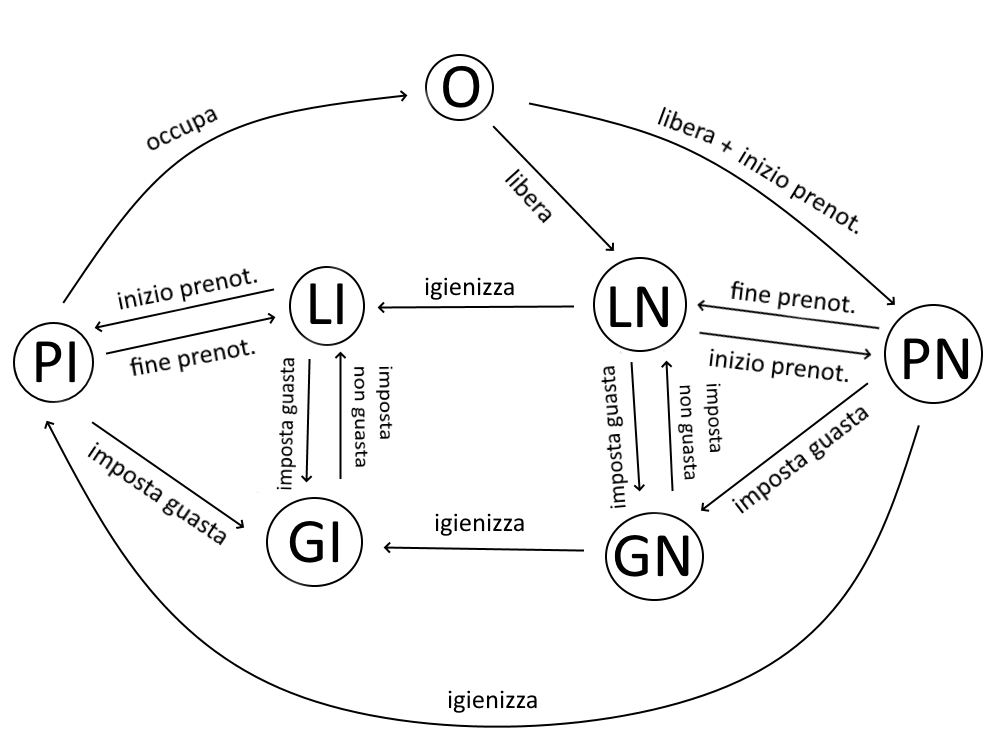
\includegraphics[width=15cm]{res/images/statipostazioni.png}
	\caption{Stati postazioni}
	\label{fig:stati postazioni}
\end{figure}
Lo schema sovrastante descrive come cambiano gli stati delle postazioni. \newline
Stati possibili:
\begin{itemize}
	\item O: occupata;
	\item LI: libera e igienizzata;
	\item LN: libera e non igienizzata;
	\item PI: prenotata e igienizzata;
	\item PN: prenotata e non igienizzata;
	\item GI: guasta e igienizzata;
	\item GN: guasta e non igienizzata.
\end{itemize}
Possibili transizioni:
\begin{itemize}
	\item occupa: un dipendente occupa la postazione;
	\item libera: un dipendente libera la postazione che stava occupando;
	\item inizio prenot.: scatta il momento di inizio di una prenotazione sulla postazione;
	\item fine prenot.: scatta il momento di fine di una prenotazione sulla postazione;
	\item libera + inizio prenot.: un utente lascia la postazione che occupava e nello stesso istante una nuova prenotazione comincia;
	\item igienizza: un addetto alle pulizie o un dipendente igienizza la postazione;
	\item imposta guasta: l'amministratore imposta la postazione come guasta;
	\item imposta non guasta: l'amministratore imposta la postazione come non guasta.
\end{itemize}

\subsection{Caratteristiche degli utenti}
Le categorie di utenti individuate nel C1 sono tre:
\begin{itemize}
	\item amministratore di un'azienda;
	\item dipendente di un'azienda o studente di un'università;
    \item addetto alle pulizie.
\end{itemize}
per tutte e tre le utenze non sono richieste conoscenze tecniche specifiche per l'utilizzo rispettivamente dell'applicazione web e di quella mobile. Nel caso di necessità, DPCM 2077 fornirà un manuale utente per poter guidare gli utenti nell'utilizzo del prodotto.
\subsection{Piattaforma d'esecuzione}
Il backend avrà il compito di interagire con Ethereum, in modo da creare una sorta di database certificato, dove registrare le varie azioni. Il frontend, sarà costituito da un'interfaccia utente sotto forma di applicazione web e app mobile. 
\subsection{Vincoli generali}
A un amministratore, per usufruire del servizio, è sufficiente un browser installato su un computer con connessione a internet; per gli utenti dell'applicazione un dispositivo con SO \glock{Android}, una connessione a internet e un tag NFC (in particolare \glock{NFC}) o in modo opzionale della tecnologia \glock{bluetooth low energy}.

